\chapter{Arhitektura i dizajn sustava}
		
		Arhitektura sustava se sastoji od tri glavna podsustava, a to su web preglednik, web poslužitelj i baza podataka.
		
		\begin{itemize}
		
		\item  \textbf{Web preglednik} je program s pomoću kojeg korisnik pristupa sustavu, odnosno sva korisnička interakcija se odvija preko web-preglednika. Korisnik putem web preglednika šalje zahtjeve za resursima, koje web preglednik dohvaća od web poslužitelja, i onda se ti resursi na ispravan način interpretiraju i prikazuju. Korisnik također može i slati podatke preko web aplikacije, najčešće korištenjem formi.
		
		\item \textbf{Web poslužitelj} je centralni dio web aplikacije. Zasniva se na protokolu HTTP, komunicira i s korisnikom i s bazom podataka, te na zahtjeve korisnika dohvaća resurse ili obrađuje podatke poslane korištenjem forme i ažurira bazu podataka.
		
		\item \textbf{Baza podataka} služi za pohranu podataka sustava. Gotovo svi scenariji korištenja web aplikacije podrazumijevaju dohvaćanje podataka iz baze, i spremanje podataka u bazu.
		\end{itemize}
		
		Aplikacija je izgrađena na principu arhitekture zasnovane na događajima, i shodno tome, aplikacija se temelji na MVC konceptu. MVC se sastoji od tri komponente:	
		
		\begin{itemize}
		
		\item \textbf{Model} sadrži razrede čiji objekti se obrađuju.
		
		\item \textbf{View} (hrv. pogled) sadrži razrede čiji objekti služe za prikaz podataka.
		
		\item \textbf{Controller} (hrv. nadglednik) sadrži razrede koji upravljaju i rukuju korisničkom interakcijom s pogledom i modelom.
		
		\end{itemize}
		
		Aplikacija je izgrađena korištenjem objektno orijentirane paradigme. Za backend je korišten radni okvir Java Spring. Za frontend je korišten React. Od vanjskih servisa, integrirana je podrška sinkronizacije događaja s Google Kalendarom.
	
		

		

				
		\section{Baza podataka}
			
			\textbf{\textit{dio 1. revizije}}\\
			
		
Naš sustav koristi relacijsku bazu podataka, za koju smo se odlučili iz jednostavnog razloga. Razlog su bili podaci koji su vrlo povezani međusobno, zbog toga koristimo relacije. Relacija, odnosno tablica, je srž i glavna komponenta baze koja se sastoji od imena i skupa atributa.Baza podataka mora biti brza i efikasna u svojoj zadaći, to jest u pohranjivanju, dohvaćanju i izmjeni podataka.\\
Naša baza podataka sastoji se od jedanaest entiteta:
\begin{multicols}{3}

\begin{itemize}
\item Account
\item Event
\item Thread
\item Post

\end{itemize}

\columnbreak

\begin{itemize}
\item District
\item Street
\item Home
\item Role

\end{itemize}

\begin{itemize}
\item RoleRequest
\item Meeting
\item Council
\end{itemize}
\end{multicols}
		
			\subsection{Opis tablica}
			
				
	\textbf{\large Account}\quad\quad Entitet Account sadržava informacije o korisniku.
				Atributi koje sadrži entitet su: Identifikacijski ključ korisnika, email, ime, prezime, password, "isBlocked" što pokazuje da li je korisnik blokiran, "isAddressValid" što pokazuje ima li korisnik ispravnu adresu na kojoj stanuje, šifru kuće u kojoj stanuje, šifru sastanaka ako je korisnik vijećnik te je prisustvovao sastanku vijeća, šifru vijeća ako je korisnik vijećnik te šifra četvrti kojoj korisnik pripada. Ovaj entitet u vezi je One-to-Many s entitetom Post preko atributa IDAccount korisnika, u vezi Many-to-One s Meeting preko IDMeeting, u vezi One-to-Many s entitetom Event preko atributa IDAccount. Također je u vezi One-to-Many s RoleRequest preko IDAccount, u vezi Many-to-One s entitetom District preko atributa IDDistrict. U vezi je Many-to-One s entitetom Home preko IDHome te naposlijetku je u vezi Many-to-Many s Role preko atributa IDAccount.
				
					
				\begin{longtblr}[
					label=none,
					entry=none
					]{
						width = \textwidth,
						colspec={|X[6,l]|X[6, l]|X[20, l]|}, 
						rowhead = 1,
					} %definicija širine tablice, širine stupaca, poravnanje i broja redaka naslova tablice
					\hline \multicolumn{3}{|c|}{\textbf{Account}}	 \\ \hline[3pt]
					\SetCell{LightGreen}IDAccount & INT	&  	Identifikacijski ključ korisnika  	\\ \hline
					email	& VARCHAR & Email korisnika  	\\ \hline
					firstName & VARCHAR & Ime korisnika \\ \hline
					lastName & VARCHAR & Prezime korisnika \\ \hline
					password & VARCHAR & Lozinka korisnika \\ \hline
					isBlocked & BOOLEAN & Oznaka je li korisnik blokiran \\ \hline
					isAddressValid & BOOLEAN & Oznaka je li adresa korisnika valjana \\ \hline
					\SetCell{LightBlue}IDHome & INT & Identifikacijski ključ korisnikove kuće  	\\ \hline
					\SetCell{LightBlue}IDMeeting	& INT & Identifikacijski ključ sastanka  	\\ \hline
					\SetCell{LightBlue}IDCouncil	 & INT & Identifikacijski ključ vijeća četvrti  	\\ \hline
					\SetCell{LightBlue}IDDistrict	& INT & Identifikacijski ključ četvrti kojoj korisnik pripada  	\\ \hline
					\end{longtblr}
					
					
	\textbf{\large Event}\quad\quad Ovaj entitet sadržava sve informacije vezane uz događaj.
		Atributi koje sadrži entitet su: Identifikacijski ključ događaja, naziv događaja, opis, trajanje, vrijeme, lokaciju te status događaja. Entitet je u samo jednoj i to Many-to-One vezi s entitetom Account preko atributa IDAccount.
					
					
					\begin{longtblr}[
					label=none,
					entry=none
					]{
						width = \textwidth,
						colspec={|X[7,l]|X[6, l]|X[20, l]|}, 
						rowhead = 1,
					} %definicija širine tablice, širine stupaca, poravnanje i broja redaka naslova tablice
					\hline \multicolumn{3}{|c|}{\textbf{Event}}	 \\ \hline[3pt]
					\SetCell{LightGreen}IDEvent & INT	&  	Identifikacijski ključ događaja  	\\ \hline
					eventName	& VARCHAR & Naziv događaja  	\\ \hline
					eventDatetime & DATETIME & Vrijeme događaja \\ \hline
					eventLocation & VARCHAR & Lokacija događaja \\ \hline
					eventDuration & INTERVAL & Trajanje događaja \\ \hline
					eventDescription & VARCHAR & Opis događaja \\ \hline
					eventStatus & VARCHAR & Status događaja \\ \hline
					\SetCell{LightBlue}IDAccount & INT & Identifikacijski ključ korisnika  	\\ \hline
				
				\end{longtblr}
				
				
	\textbf{\large Thread}\quad\quad	Ovaj entitet sadržava sve informacije vezane uz dretvu na forumu. Sadrži atribute: Identifikacijski ključ dretve, ime dretve te šifru četvrti kako bi se utvrdilo kojem forumu pripada ta dretva, odnosno četvrti. Ovaj entitet je u One-to-One vezi s entitetom Meeting preko atributa IDThread te je u vezi One-to-Many s District preko šifre četvrti.
				
				\begin{longtblr}[
					label=none,
					entry=none
					]{
						width = \textwidth,
						colspec={|X[6,l]|X[6, l]|X[20, l]|}, 
						rowhead = 1,
					} %definicija širine tablice, širine stupaca, poravnanje i broja redaka naslova tablice
					\hline \multicolumn{3}{|c|}{\textbf{Thread}}	 \\ \hline[3pt]
					\SetCell{LightGreen}IDThread & INT	&  	Identifikacijski ključ dretve  	\\ \hline
					threadName	& VARCHAR & Ime dretve  	\\ \hline 
					\SetCell{LightBlue} IDDistrict	& INT & Identifikacijski ključ četvrti  	\\ \hline 
				\end{longtblr}
				
	\textbf{\large Post}\quad\quad Ovaj entitet sadržava sve informacije vezane uz objavu na forumu. Sadrži atribute: Identifikacijski ključ objave, vrijeme objave, sadržaj objave, šifra odgovora na objavu(ako postoji), šifra dretve kojoj objava pripada te šifra korisnika koji je objavio objavu. Ovaj entitet je u dvije Many-to-One veze i to s entitetima Account i Thread preko njihovih odgovarajućih identifikacijskih šifri(IDAccount i IDThread).
				
				
					\begin{longtblr}[
					label=none,
					entry=none
					]{
						width = \textwidth,
						colspec={|X[6,l]|X[6, l]|X[20, l]|}, 
						rowhead = 1,
					} %definicija širine tablice, širine stupaca, poravnanje i broja redaka naslova tablice
					\hline \multicolumn{3}{|c|}{\textbf{Post}}	 \\ \hline[3pt]
					\SetCell{LightGreen}IDPost & INT	&  	Identifikacijski ključ objave  	\\ \hline
					postDatetime	& DATETIME & Vrijeme postavljanja objave  	\\ \hline
					postContent & VARCHAR & Sadržaj objave \\ \hline
					replyId & INT & Identifikacijski ključ odgovora na objavu \\ \hline
					\SetCell{LightBlue}IdThread	 & INT & Identifikacijski ključ pripadajuće dretve  	\\ \hline
					\SetCell{LightBlue}IDAccount	& INT & Identifikacijski ključ korisnika koji je objavio objavu  	\\ \hline
				\end{longtblr}
				
				
	\textbf{\large District}\quad\quad Ovaj entitet sadržava sve informacije vezane uz četvrt. Sadrži atribute: Identifikacijski ključ četvrti te naziv četvrti. Ovaj entitet je u tri One-to-Many veze i to s entitetima Account, Post i Street preko vlastite identifikacijske šifre(IDDistrict). Također je u One-to-One vezi sa slabim entitetom Council preko atributa IDDistrict.
				
					\begin{longtblr}[
					label=none,
					entry=none
					]{
						width = \textwidth,
						colspec={|X[6,l]|X[6, l]|X[20, l]|}, 
						rowhead = 1,
					} %definicija širine tablice, širine stupaca, poravnanje i broja redaka naslova tablice
					\hline \multicolumn{3}{|c|}{\textbf{District}}	 \\ \hline[3pt]
					\SetCell{LightGreen}IDDistrict & INT	&  	Identifikacijski ključ četvrti  	\\ \hline
					districtName	& INT & Naziv četvrti  	\\ \hline
				\end{longtblr}
				
				\textbf{\large Street}\quad\quad Ovaj entitet sadržava sve informacije vezane uz ulicu. Sadrži atribute: Identifikacijski ključ ulice, naziv ulice, najmanji kućanski broj u ulici, najveći kućanski broj u ulici te šifra četvrti u kojoj se ulica nalazi. Ovaj entitet je u Many-to-One vezi s entitetom District preko šifre četvrti. Također je u One-to-Many vezi s entitetom Home preko atributa IDStreet.
				
					\begin{longtblr}[
					label=none,
					entry=none
					]{
						width = \textwidth,
						colspec={|X[10,l]|X[6, l]|X[20, l]|}, 
						rowhead = 1,
					} %definicija širine tablice, širine stupaca, poravnanje i broja redaka naslova tablice
					\hline \multicolumn{3}{|c|}{\textbf{Street}}	 \\ \hline[3pt]
					\SetCell{LightGreen}IDStreet & INT	&  	Identifikacijski ključ ulice  	\\ \hline
					streetName	& VARCHAR & Naziv ulice  	\\ \hline
					minStreetNumber & INT & Najmanji kućanski broj ulice \\ \hline
					maxStreetNumber & INT & Najveći kućanski broj ulice \\ \hline
					\SetCell{LightBlue}IDDistrict	 & INT & Identifikacijski ključ pripadajuće četvrti  	\\ \hline
					\end{longtblr}
					
					
	\textbf{\large Home}\quad\quad Ovaj entitet sadržava sve informacije vezane uz kuću korisnika. Sadrži atribute: Identifikacijski ključ kuće, kućni broj te šifra ulice u kojoj se kuća nalazi. Ovaj entitet je u Many-to-One vezi s entitetom Steet preko šifre ulice. Također je u One-to-Many vezi s entitetom Account preko atributa IDAccount.
					
					
							
					\begin{longtblr}[
					label=none,
					entry=none
					]{
						width = \textwidth,
						colspec={|X[6,l]|X[6, l]|X[20, l]|}, 
						rowhead = 1,
					} %definicija širine tablice, širine stupaca, poravnanje i broja redaka naslova tablice
					\hline \multicolumn{3}{|c|}{\textbf{Home}}	 \\ \hline[3pt]
					\SetCell{LightGreen}IDHome & INT	&  	Identifikacijski ključ kuće  	\\ \hline
					homeNumber	& INT & Kućanski broj  	\\ \hline
					\SetCell{LightBlue}IDStreet	 & INT & Identifikacijski ključ pripadajuće ulice  	\\ \hline
							\end{longtblr}
							
							
							
	\textbf{\large Role}\quad\quad Ovaj entitet sadržava sve informacije vezane uz ulogu korisnika. Sadrži atribute: Identifikacijski ključ uloge te naziv uloge. Ovaj entitet je u Many-to-Many vezi s entitetom Account preko šifre uloge te u One-to-Many vezi s entitetom RoleRequest preko šifre uloge.
							
							\begin{longtblr}[
					label=none,
					entry=none
					]{
						width = \textwidth,
						colspec={|X[6,l]|X[6, l]|X[20, l]|}, 
						rowhead = 1,
					} %definicija širine tablice, širine stupaca, poravnanje i broja redaka naslova tablice
					\hline \multicolumn{3}{|c|}{\textbf{Role}}	 \\ \hline[3pt]
					\SetCell{LightGreen}IDRole & INT	&  	Identifikacijski ključ uloge  	\\ \hline
					roleName	& VARCHAR & Naziv uloge 	\\ \hline
					
							\end{longtblr}
							
							
							\textbf{\large RoleRequest}\quad\quad Ovaj entitet sadržava sve informacije vezane uz zahtjev korisnika za ulogom. Sadrži atribute: Identifikacijski ključ zahtjeva, status zahtjeva te šifra korisnika koji je podnio zahtjev i šifra uloge koju korisnik zahtjeva. Ovaj entitet je u Many-to-One vezi s entitetom Role preko šifre uloge. Također je u Many-to-One vezi s entitetom Account preko atributa IDAccount.			
							\begin{longtblr}[
					label=none,
					entry=none
					]{
						width = \textwidth,
						colspec={|X[8,l]|X[6, l]|X[20, l]|}, 
						rowhead = 1,
					} %definicija širine tablice, širine stupaca, poravnanje i broja redaka naslova tablice
					\hline \multicolumn{3}{|c|}{\textbf{RoleRequest}}	 \\ \hline[3pt]
					\SetCell{LightGreen}IDRoleRequest & INT	&  	Identifikacijski ključ zahtjeva za ulogu  	\\ \hline
					roleRequestStatus	& VARCHAR & Status zahtjeva za ulogu  	\\ \hline
					\SetCell{LightBlue}IDAccount	 & INT & Identifikacijski ključ korisnika 	\\ \hline
					\SetCell{LightBlue}IDRole	 & INT & Identifikacijski ključ uloge  	\\ \hline
							\end{longtblr}
							
\textbf{\large AccountRole}\quad\quad Ova join tablica koja je posljedično nastala spajanjem entiteta Account s entitetom Role vezom Many-to-Many sadržava informacije o ulozi korisnika. Sadrži 2 atributa koja su ključ entiteta Account i ključ entiteta Role.	
							
								\begin{longtblr}[
					label=none,
					entry=none
					]{
						width = \textwidth,
						colspec={|X[7,l]|X[6, l]|X[20, l]|}, 
						rowhead = 1,
					} %definicija širine tablice, širine stupaca, poravnanje i broja redaka naslova tablice
					\hline \multicolumn{3}{|c|}{\textbf{AccountRole}}	 \\ \hline[3pt]
					\SetCell{LightGreen}\underline{IDAccount} & INT	&  	Identifikacijski ključ korisnika  	\\ \hline
					\SetCell{LightGreen}\underline{IDRole}	 & INT & Identifikacijski ključ uloge \\ \hline

					  	
							\end{longtblr}
							
							
						\textbf{\large Meeting}\quad\quad Ovaj slabi entitet sadržava sve informacije vezane uz sastanak vijeća. Sadrži atribute: Identifikacijski ključ sastanka, naziv sastanka, izvještaj te šifru autora izvještaja. Također sadrži šifru vijeća, šifru četvrti te šifru dretve na forumu ukoliko je otvorena na temu izvještaja. Ovaj entitet je u One-to-One vezi s entitetom Thread preko šifre dretve. Također je u Many-to-One vezi sa slabim entitetom Council preko šifre vijeća te u vezi	One-to-Many s entitetom Account preko šifre sastanka.
							
							
							\begin{longtblr}[
					label=none,
					entry=none
					]{
						width = \textwidth,
						colspec={|X[7,l]|X[6, l]|X[20, l]|}, 
						rowhead = 1,
					} %definicija širine tablice, širine stupaca, poravnanje i broja redaka naslova tablice
					\hline \multicolumn{3}{|c|}{\textbf{Meeting}}	 \\ \hline[3pt]
					\SetCell{LightGreen}IDMeeting & INT	&  	Identifikacijski ključ sastanka  	\\ \hline
					\SetCell{LightGreen}\underline{IDCounil}	 & INT & Identifikacijski ključ vijeća \\ \hline
					\SetCell{LightGreen}\underline{IDDistrict}	 & INT & Identifikacijski ključ četvrti \\ \hline
					\SetCell{LightBlue}IDThread	 & INT & Identifikacijski ključ dretve \\ \hline
					meetingReport	& VARCHAR & Izvješće sastanka  	\\ \hline
					reportAuthorId	& INT & Identifikacijski broj korisnika koji je sastavio izvješće\\ \hline
					meetingTitle & VARCHAR & Naziv sastanka \\ \hline 
					  	
							\end{longtblr}
							
							
							
							\textbf{\large Council}\quad\quad Ovaj slabi entitet sadržava sve informacije vezane uz vijeće. Sadrži atribute: Identifikacijski ključ vijeća te šifru četvrti kojoj pripada. Ovaj entitet je u One-to-One vezi s entitetom District preko šifre četvrti. Također je u One-to-Many vezi sa slabim entitetom Meeting preko šifre vijeća.
							
							\begin{longtblr}[
					label=none,
					entry=none
					]{
						width = \textwidth,
						colspec={|X[6,l]|X[6, l]|X[20, l]|}, 
						rowhead = 1,
					} %definicija širine tablice, širine stupaca, poravnanje i broja redaka naslova tablice
					\hline \multicolumn{3}{|c|}{\textbf{Council}}	 \\ \hline[3pt]
					\SetCell{LightGreen}IDCouncil & INT	&  	Identifikacijski ključ vijeća  	\\ \hline
					\SetCell{LightGreen}\underline{IDDistrict}	 & INT & Identifikacijski ključ četvrti  	\\ \hline
							\end{longtblr}
							
							
			\eject	
			
			\subsection{Dijagram baze podataka}
	\begin{figure}[h]
	\centering
  \hbox{\hspace{-2.2cm}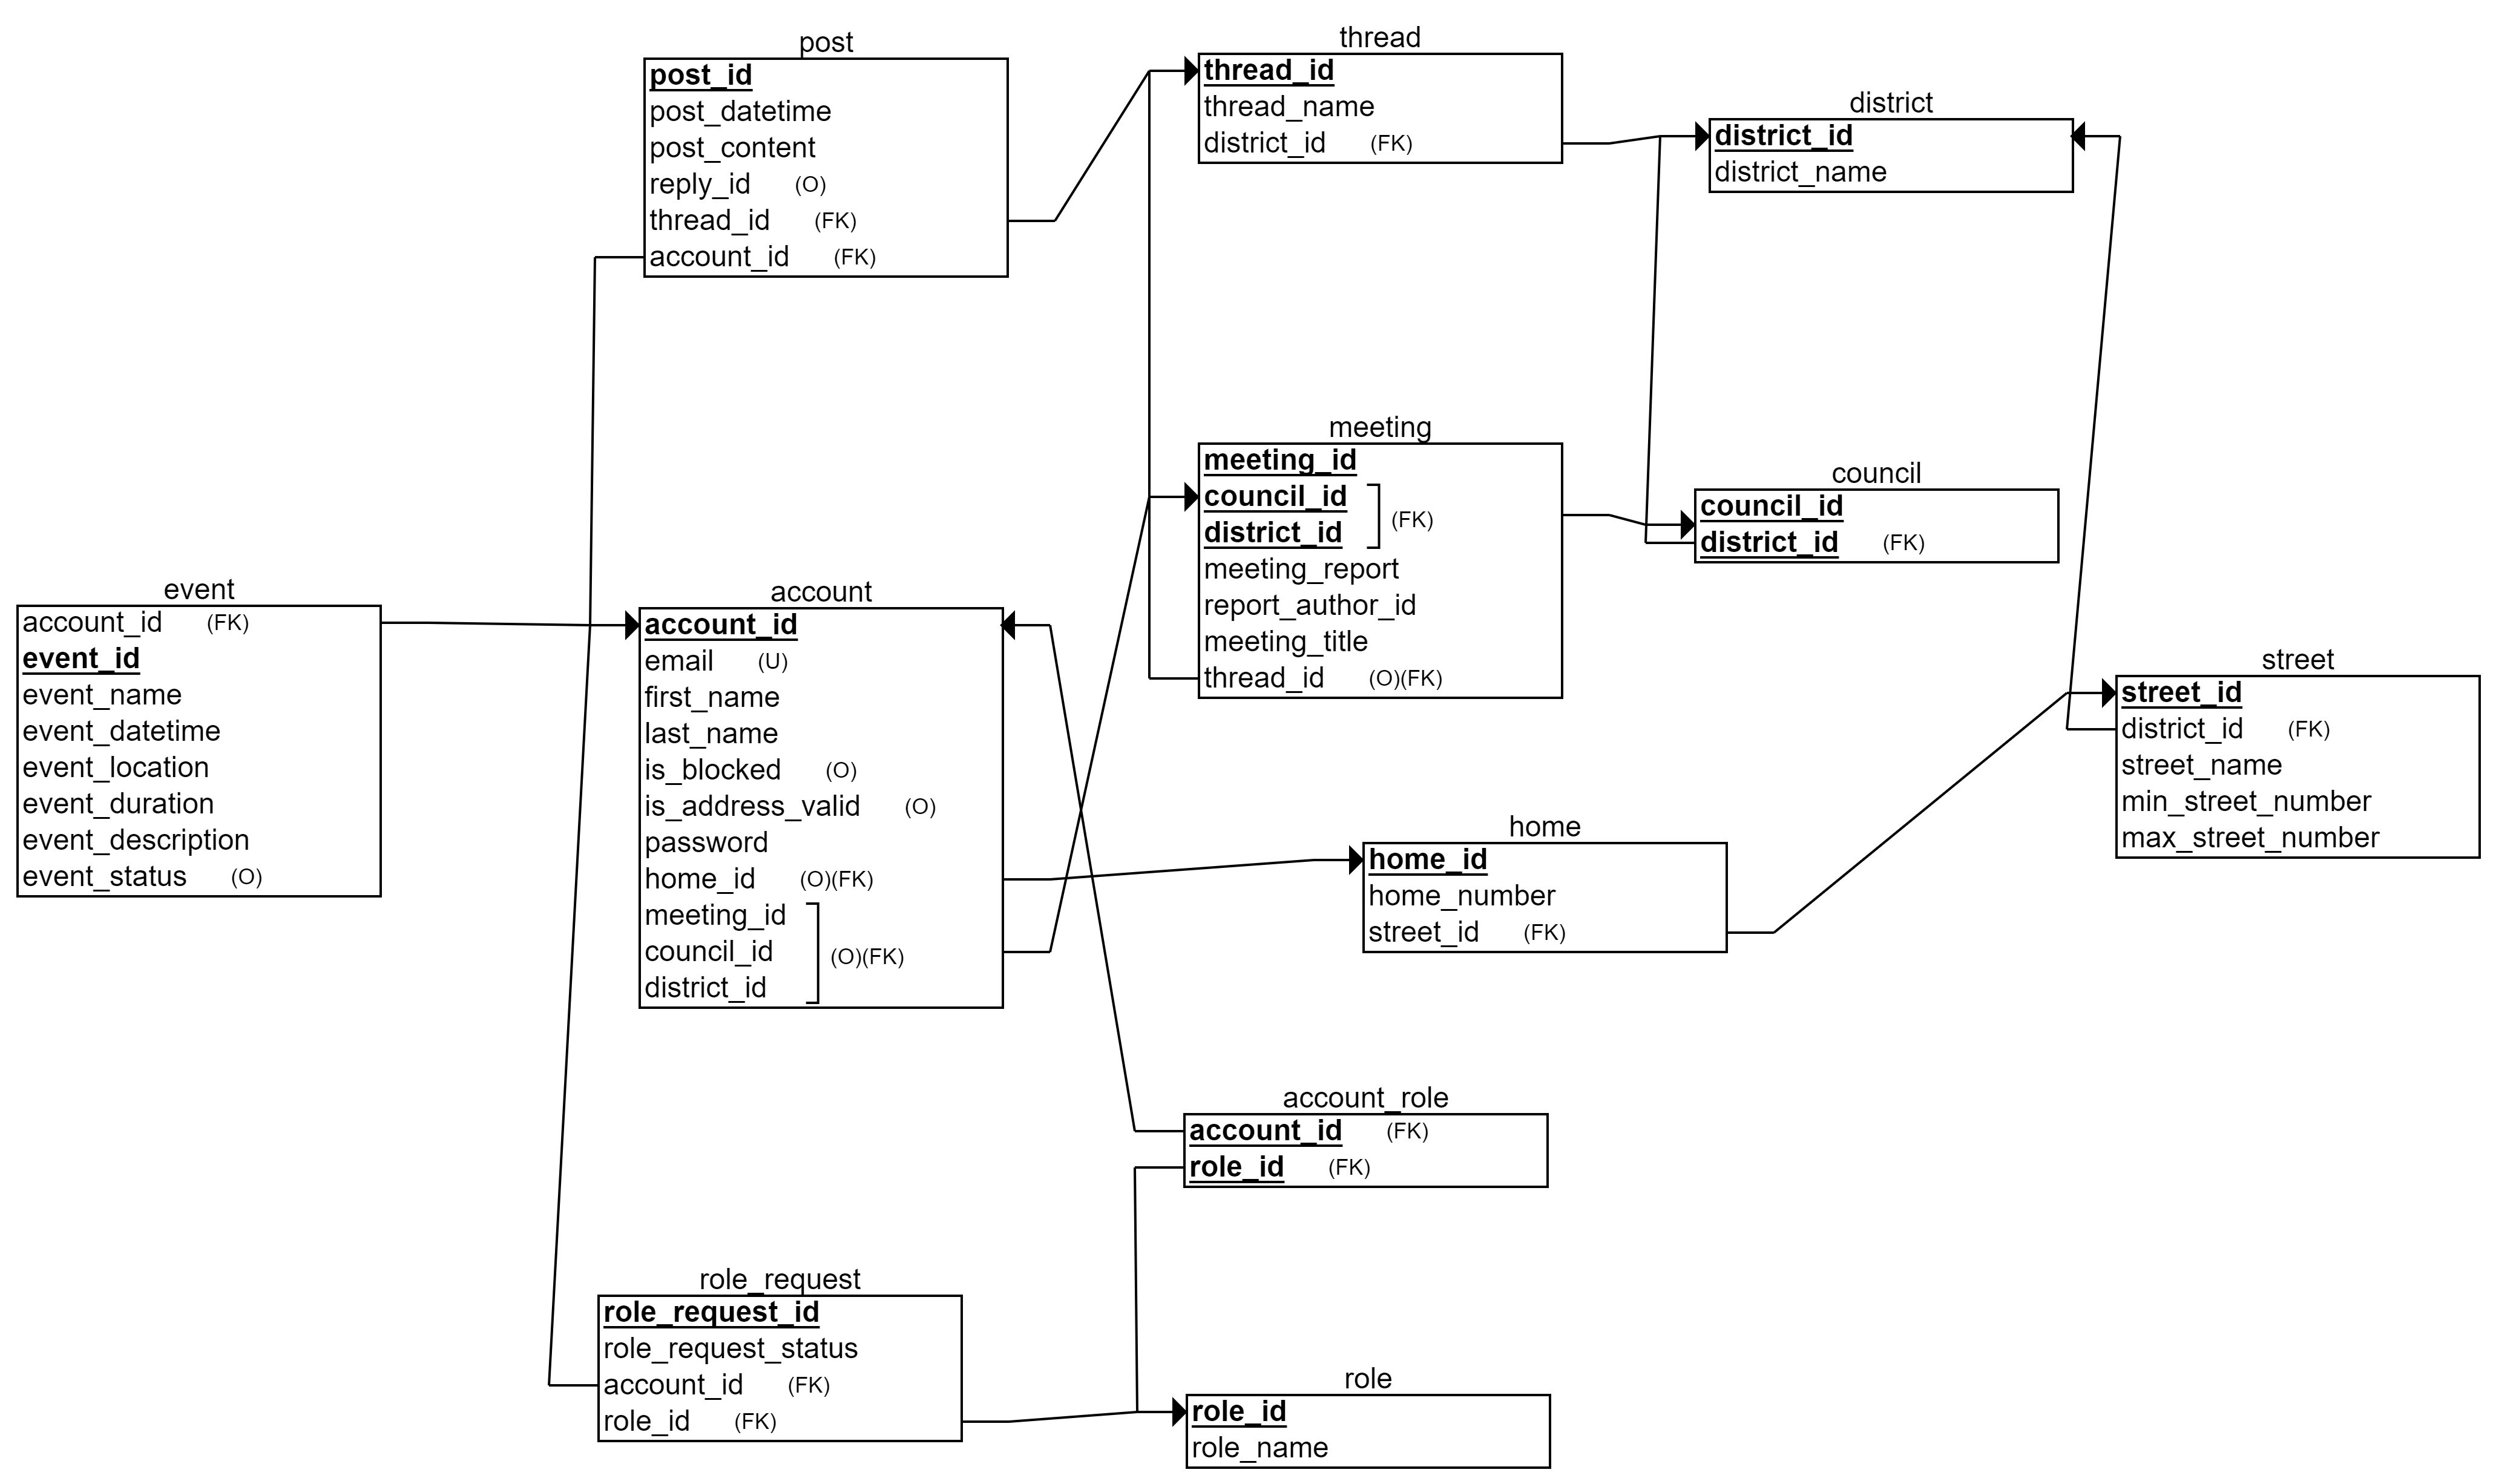
\includegraphics[width = 200mm,scale = 3]{Dijagram_11.png}}
  \caption{Relacijska shema}
  \label{Relacijska_shema}
\end{figure}
			
			\eject
			
		\section{Dijagram razreda}
		
			\textit{Potrebno je priložiti dijagram razreda s pripadajućim opisom. Zbog preglednosti je moguće dijagram razlomiti na više njih, ali moraju biti grupirani prema sličnim razinama apstrakcije i srodnim funkcionalnostima.}\\
			
			\textbf{\textit{dio 1. revizije}}\\
			
			\textit{Prilikom prve predaje projekta, potrebno je priložiti potpuno razrađen dijagram razreda vezan uz \textbf{generičku funkcionalnost} sustava. Ostale funkcionalnosti trebaju biti idejno razrađene u dijagramu sa sljedećim komponentama: nazivi razreda, nazivi metoda i vrste pristupa metodama (npr. javni, zaštićeni), nazivi atributa razreda, veze i odnosi između razreda.}\\
			
			\textbf{\textit{dio 2. revizije}}\\			
			
			\textit{Prilikom druge predaje projekta dijagram razreda i opisi moraju odgovarati stvarnom stanju implementacije}
			
			
			
			\eject
		
		\section{Dijagram stanja}
			
			
			\textbf{\textit{dio 2. revizije}}\\
			
			\textit{Potrebno je priložiti dijagram stanja i opisati ga. Dovoljan je jedan dijagram stanja koji prikazuje \textbf{značajan dio funkcionalnosti} sustava. Na primjer, stanja korisničkog sučelja i tijek korištenja neke ključne funkcionalnosti jesu značajan dio sustava, a registracija i prijava nisu. }
			
			
			\eject 
		
		\section{Dijagram aktivnosti}
			
			\textbf{\textit{dio 2. revizije}}\\
			
			 \textit{Potrebno je priložiti dijagram aktivnosti s pripadajućim opisom. Dijagram aktivnosti treba prikazivati značajan dio sustava.}
			
			\eject
		\section{Dijagram komponenti}
		
			\textbf{\textit{dio 2. revizije}}\\
		
			 \textit{Potrebno je priložiti dijagram komponenti s pripadajućim opisom. Dijagram komponenti treba prikazivati strukturu cijele aplikacije.}
